\def\bmode{0} % Mode 0 for presentation, mode 1 for a handout with notes, mode 2 for handout without notes
\if 0\bmode
\documentclass[smaller]{beamer}
\else \if 1\bmode
\immediate\write18{pdflatex -jobname=\jobname-Handout-Notes\space\jobname}
\documentclass[smaller,handout]{beamer}
\usepackage{handoutWithNotes}
\pgfpagesuselayout{2 on 1 with notes}[letterpaper, landscape, border shrink=4mm]
\else \if 2\bmode
\immediate\write18{pdflatex -jobname=\jobname-Handout\space\jobname}
\documentclass[smaller,handout]{beamer}
\fi
\fi
\fi

% \documentclass[smaller,handout]{beamer}

% \usepackage[T1]{fontenc} 
% \usepackage{lmodern} 
%\usepackage{etex}
 %\newcommand{\num}{6{} }

% \usetheme[
%   outer/progressbar=foot,
%   outer/numbering=fraction,
%   block=fill,
%   inner/subsectionpage=progressbar
% ]{metropolis}
\usetheme{Madrid}
\useoutertheme[subsection=false]{miniframes} % Alternatively: miniframes, infolines, split
\useinnertheme{circles}
% %\useoutertheme{Frankfurt}
% \usecolortheme{beaver}
% %\useoutertheme{crane}
% %\useoutertheme{metropolis}
\usepackage[backend=biber,style=authoryear,maxcitenames=2,maxbibnames=99,safeinputenc,url=false, eprint=false]{biblatex}
%\addbibresource{bib/references.bib}
% \AtEveryCitekey{\iffootnote{{\tiny}\tiny}{\tiny}}

% %\usepackage{pgfpages}
% %\setbeameroption{hide notes} % Only slides
% %\setbeameroption{show only notes} % Only notes
% %\setbeameroption{hide notes} % Only notes
% %\setbeameroption{show notes on second screen=right} % Both

% % \usepackage[sfdefault]{Fira Sans}

% % \setsansfont[BoldFont={Fira Sans}]{Fira Sans Light}
% % \setmonofont{Fira Mono}

% %\usepackage{fira}
% %\setsansfont{Fira}
% %\setmonofont{Fira Mono}
% % To give a presentation with the Skim reader (http://skim-app.sourceforge.net) on OSX so
% % that you see the notes on your laptop and the slides on the projector, do the following:
% % 
% % 1. Generate just the presentation (hide notes) and save to slides.pdf
% % 2. Generate onlt the notes (show only nodes) and save to notes.pdf
% % 3. With Skim open both slides.pdf and notes.pdf
% % 4. Click on slides.pdf to bring it to front.
% % 5. In Skim, under "View -> Presentation Option -> Synhcronized Noted Document"
% %    select notes.pdf.
% % 6. Now as you move around in slides.pdf the notes.pdf file will follow you.
% % 7. Arrange windows so that notes.pdf is in full screen mode on your laptop
% %    and slides.pdf is in presentation mode on the projector.

% % Give a slight yellow tint to the notes page
% \setbeamertemplate{note page}{\pagecolor{yellow!5}\insertnote}\usepackage{palatino}

% %\usetheme{metropolis}
% %\usecolortheme{beaver}
 \usepackage{tipa}
% \usepackage{enumerate}
% \definecolor{darkcandyapplered}{HTML}{A40000}
% \definecolor{lightcandyapplered}{HTML}{e74c3c}

% %\setbeamercolor{title}{fg=darkcandyapplered}

% \definecolor{UBCblue}{rgb}{0.04706, 0.13725, 0.26667} % UBC Blue (primary)
% \definecolor{UBCgrey}{rgb}{0.3686, 0.5255, 0.6235} % UBC Grey (secondary)

% % \setbeamercolor{palette primary}{bg=darkcandyapplered,fg=white}
% % \setbeamercolor{palette secondary}{bg=darkcandyapplered,fg=white}
% % \setbeamercolor{palette tertiary}{bg=darkcandyapplered,fg=white}
% % \setbeamercolor{palette quaternary}{bg=darkcandyapplered,fg=white}
% % \setbeamercolor{structure}{fg=darkcandyapplered} % itemize, enumerate, etc
% % \setbeamercolor{section in toc}{fg=darkcandyapplered} % TOC sections
% % \setbeamercolor{frametitle}{fg=darkcandyapplered,bg=white} % TOC sections
% % \setbeamercolor{title in head/foot}{bg=white,fg=white} % TOC sections
% % \setbeamercolor{button}{fg=darkcandyapplered} % TOC sections

% % % Override palette coloring with secondary
% % \setbeamercolor{subsection in head/foot}{bg=lightcandyapplered,fg=white}

%\usecolortheme{crane}
% \makeatletter
% \setbeamertemplate{headline}{%
%   \begin{beamercolorbox}[colsep=1.5pt]{upper separation line head}
%   \end{beamercolorbox}
%   \begin{beamercolorbox}{section in head/foot}
%     \vskip1pt\insertsectionnavigationhorizontal{\paperwidth}{}{}\vskip1pt
%   \end{beamercolorbox}%
%   \ifbeamer@theme@subsection%
%     \begin{beamercolorbox}[colsep=1.5pt]{middle separation line head}
%     \end{beamercolorbox}
%     \begin{beamercolorbox}[ht=2.5ex,dp=1.125ex,%
%       leftskip=.3cm,rightskip=.3cm plus1fil]{subsection in head/foot}
%       \usebeamerfont{subsection in head/foot}\insertsubsectionhead
%     \end{beamercolorbox}%
%   \fi%
%   \begin{beamercolorbox}[colsep=1.5pt]{lower separation line head}
%   \end{beamercolorbox}
% }
% \makeatother

% Reduce size of frame box
\setbeamertemplate{frametitle}{%
    \nointerlineskip%
    \begin{beamercolorbox}[wd=\paperwidth,ht=2.0ex,dp=0.6ex]{frametitle}
        \hspace*{1ex}\insertframetitle%
    \end{beamercolorbox}%
}


%\setbeamercolor{frametitle}{bg=darkcandyapplered!80!black!90!white}
%\setbeamertemplate{frametitle}{\bf\insertframetitle}

%\setbeamercolor{footnote mark}{fg=darkcandyapplered}
%\setbeamercolor{footnote}{fg=darkcandyapplered!70}
%\Raggedbottom
%\setbeamerfont{page number in head/foot}{size=\tiny}
%\usepackage[tracking]{microtype}


% %\usepackage[sc,osf]{mathpazo}   % With old-style figures and real smallcaps.
% %\linespread{1.025}              % Palatino leads a little more leading

% % Euler for math and numbers
% %\usepackage[euler-digits,small]{eulervm}
% %\AtBeginDocument{\renewcommand{\hbar}{\hslash}}
\usepackage{graphicx,multirow,booktabs}


% %\mode<presentation> { \setbeamercovered{transparent} }

\setbeamertemplate{navigation symbols}{}
\makeatletter
\def\beamerorig@set@color{%
  \pdfliteral{\current@color}%
  \aftergroup\reset@color
}
\def\beamerorig@reset@color{\pdfliteral{\current@color}}
\makeatother


% %=== GRAPHICS PATH ===========
\graphicspath{{./images/}}
% % Marginpar width
% %Marginpar width
% %\setlength{\marginparsep}{.02in}


% %% Captions
% % \usepackage{caption}
% % \captionsetup{
% %   labelsep=quad,
% %   justification=raggedright,
% %   labelfont=sc
% % }

% \setbeamerfont{caption}{size=\footnotesize}
% \setbeamercolor{caption name}{fg=darkcandyapplered}

% %AMS-TeX packages

\usepackage{amssymb,amsmath,amsthm,mathtools}
\DeclareMathOperator*{\argmax}{arg\,max}
\DeclareMathOperator*{\argmin}{arg\,min}
\usepackage{bm}
% \usepackage{color}

% %https://tex.stackexchange.com/a/31370/2269
% \usepackage{mathtools,cancel}

% \renewcommand{\CancelColor}{\color{red}} %change cancel color to red

% \makeatletter
% \let\my@cancelto\cancelto %copy over the original cancelto command
% \newcommand<>{\cancelto}[2]{\alt#3{\my@cancelto{#1}{#2}}{\mathrlap{#2}\phantom{\my@cancelto{#1}{#2}}}}
% % redefine the cancelto command, using \phantom to assure that the
% % result doesn't wiggle up and down with and without the arrow
% \makeatother


% %\usepackage{comment}
% %\usepackage{hyperref,enumerate}
% \usepackage{minitoc,array}

% \definecolor{slblue}{rgb}{0,.3,.62}
% % \hypersetup{
% %     colorlinks,%
% %     citecolor=blue,%
% %     filecolor=blue,%
% %     linkcolor=blue,
% %     urlcolor=slblue
% % }

% \usepackage{epstopdf}
% \epstopdfDeclareGraphicsRule{.gif}{png}{.png}{convert gif:#1 png:\OutputFile}
% \AppendGraphicsExtensions{.gif}

% %\usepackage{listings}

% %%% TIKZ
% \usepackage{forest}
\usepackage{tikz}
\usepackage{pgfplots}
\usepackage{pgfplotstable}
%\usepackage{pgfgantt}
\pgfplotsset{compat=newest}

\usetikzlibrary{fit,arrows,shapes,positioning,shapes.geometric}
\usetikzlibrary{decorations.markings}
\usetikzlibrary{shadows,automata}
\usetikzlibrary{patterns}
\usetikzlibrary{trees,mindmap,backgrounds}
%\usetikzlibrary{circuits.ee.IEC}
\usetikzlibrary{decorations.text}
% % For Sagnac Picture
% \usetikzlibrary{%
%     decorations.pathreplacing,%
%     decorations.pathmorphing%
% }
% \tikzset{no shadows/.style={general shadow/.style=}}
% %
% %\usepackage{paralist}

% \tikzset{
%   font=\Large\sffamily\bfseries,
%   red arrow/.style={
%     midway,red,sloped,fill, minimum height=3cm, single arrow, single arrow head extend=.5cm, single arrow head indent=.25cm,xscale=0.3,yscale=0.15,
%     allow upside down
%   },
%   black arrow/.style 2 args={-stealth, shorten >=#1, shorten <=#2},
%   black arrow/.default={1mm}{1mm},
%   tree box/.style={draw, rounded corners, inner sep=1em},
%   node box/.style={white, draw=black, text=black, rectangle, rounded corners},
% }

% %%% FORMAT PYTHON CODE
% %\usepackage{listings}
% % Default fixed font does not support bold face
% \DeclareFixedFont{\ttb}{T1}{txtt}{bx}{n}{8} % for bold
% \DeclareFixedFont{\ttm}{T1}{txtt}{m}{n}{8}  % for normal

% % Custom colors
% \definecolor{deepblue}{rgb}{0,0,0.5}
% \definecolor{deepred}{rgb}{0.6,0,0}
% \definecolor{deepgreen}{rgb}{0,0.5,0}

% %\usepackage{animate}

% % Python style for highlighting
% % \newcommand\pythonstyle{\lstset{
% % language=Python,
% % basicstyle=\footnotesize\ttm,
% % otherkeywords={self},             % Add keywords here
% % keywordstyle=\footnotesize\ttb\color{deepblue},
% % emph={MyClass,__init__},          % Custom highlighting
% % emphstyle=\footnotesize\ttb\color{deepred},    % Custom highlighting style
% % stringstyle=\color{deepgreen},
% % frame=tb,                         % Any extra options here
%     % showstringspaces=false            % 
% % }}

% % % Python environment
% % \lstnewenvironment{python}[1][]
% % {
% % \pythonstyle
% % \lstset{#1}
% % }
% % {}

% % % Python for external files
% % \newcommand\pythonexternal[2][]{{
% % \pythonstyle
% % \lstinputlisting[#1]{#2}}}

% % Python for inline
% % 
% % \newcommand\pythoninline[1]{{\pythonstyle\lstinline!#1!}}

% %\usepackage{algorithm2e}

\newcommand{\eps}{\epsilon}
\newcommand{\bX}{\mb X}
\newcommand{\by}{\mb y}
\newcommand{\bbe}{\bm\beta}
\newcommand{\beps}{\bm\epsilon}
\newcommand{\bY}{\mb Y}

\newcommand{\osn}{\oldstylenums}
\newcommand{\dg}{^{\circ}}
\newcommand{\lt}{\left}
\newcommand{\rt}{\right}
\newcommand{\pt}{\phantom}
\newcommand{\tf}{\therefore}
\newcommand{\?}{\stackrel{?}{=}}
\newcommand{\fr}{\frac}
\newcommand{\dfr}{\dfrac}
\newcommand{\ul}{\underline}
\newcommand{\tn}{\tabularnewline}
\newcommand{\nl}{\newline}
\newcommand\relph[1]{\mathrel{\phantom{#1}}}
\newcommand{\cm}{\checkmark}
\newcommand{\ol}{\overline}
\newcommand{\rd}{\color{red}}
\newcommand{\bl}{\color{blue}}
\newcommand{\pl}{\color{purple}}
\newcommand{\og}{\color{orange!90!black}}
\newcommand{\gr}{\color{green!40!black}}
\newcommand{\dca}{\color{darkcandyapplered}}
\newcommand{\nin}{\noindent}
\newcommand*\circled[1]{\tikz[baseline=(char.base)]{
            \node[shape=circle,draw,thick,inner sep=1pt] (char) {\small #1};}}

\newcommand{\bc}{\begin{compactenum}[\quad--]}
\newcommand{\ec}{\end{compactenum}}

\newcommand{\p}{\partial}
\newcommand{\pd}[2]{\frac{\partial{#1}}{\partial{#2}}}
\newcommand{\dpd}[2]{\dfrac{\partial{#1}}{\partial{#2}}}
\newcommand{\pdd}[2]{\frac{\partial^2{#1}}{\partial{#2}^2}}
\newcommand{\pde}[3]{\frac{\partial^2{#1}}{\partial{#2}\partial{#3}}}
\newcommand{\nmfr}[3]{\Phi\left(\frac{{#1} - {#2}}{#3}\right)}
\newcommand{\Err}{\text{Err}}
\newcommand{\err}{\text{err}}

%\DeclarePairedDelimiter\ceil{\lceil}{\rceil}
%\DeclarePairedDelimiter\floor{\lfloor}{\rfloor}

%%%% GREEK LETTER SHORTCUTS %%%%%
\newcommand{\la}{\lambda}
\renewcommand{\th}{\theta}
\newcommand{\al}{\alpha}
\newcommand{\G}{\Gamma}
\newcommand{\si}{\sigma}
\newcommand{\Si}{\Sigma}


\pgfmathdeclarefunction{poiss}{1}{%
  \pgfmathparse{(#1^x)*exp(-#1)/(x!)}%
  }

\pgfmathdeclarefunction{gauss}{2}{%
  \pgfmathparse{1/(#2*sqrt(2*pi))*exp(-((x-#1)^2)/(2*#2^2))}%
}

\pgfmathdeclarefunction{expo}{2}{%
  \pgfmathparse{#1*exp(-#1*#2)}%
}

\pgfmathdeclarefunction{expocdf}{2}{%
  \pgfmathparse{1 -exp(-#1*#2)}%
}


% \usepackage{pst-plot}

% \usepackage{pstricks-add}
% \usepackage{auto-pst-pdf}   

% \psset{unit = 3}

% \def\target(#1,#2){%
%  {\psset{fillstyle = solid}
%   \rput(#1,#2){%
%     \pscircle[fillcolor = white](0.7,0.7){0.7}
%     \pscircle[fillcolor = blue!60](0.7,0.7){0.5}
%     \pscircle[fillcolor = white](0.7,0.7){0.3}
%     \pscircle[fillcolor = red!80](0.7,0.7){0.1}}}}
% \def\dots[#1](#2,#3){%
%     \psRandom[
%       dotsize = 2pt,
%       randomPoints = 25
%     ](!#2 #1 0.04 sub sub #3 #1 0.04 sub sub)%
%      (!#2 #1 0.04 sub add #3 #1 0.04 sub add)%
%      {\pscircle[linestyle = none](#2,#3){#1}}}


%%%%%%%%%%%%%%%%%%%%%%%%%%%%%%%%%%%%%%%%%%%%%%%%%%%
%%%%%%%%%%%%%%%%%%%%%%%%%%%%%%%%%%%%%%%%%%%%%%%%%%%
\title[CEE 697M 1d: Decision \& Information Theories]{ {\normalsize CEE 697M:  Big Data  and Machine Learning for Engineers}
  \\ Lecture 1d: Decision and Information Theories}
\date[\today]{\footnotesize \today}
\author{{\bf Jimi Oke}}
\institute[UMass Amherst]{
%\titlegraphic{\hfill
  \begin{tikzpicture}[baseline=(current bounding box.center)]
    \node[anchor=base] at (-7,0) (its) {
\includegraphics[scale=.3]{UMassEngineering_vert}} ;
  \end{tikzpicture}
  % \hfill\includegraphics[height=1.5cm]{logo}
}

%https://tex.stackexchange.com/questions/55806/mindmap-tikzpicture-in-beamer-reveal-step-by-step
  \tikzset{
    invisible/.style={opacity=0},
    visible on/.style={alt={#1{}{invisible}}},
    alt/.code args={<#1>#2#3}{%
      \alt<#1>{\pgfkeysalso{#2}}{\pgfkeysalso{#3}} % \pgfkeysalso doesn't change the path
    },
  }


% https://tex.stackexchange.com/questions/446468/labels-with-arrows-for-an-equation
% https://tex.stackexchange.com/a/402466/121799
\newcommand{\tikzmark}[3][]{
\ifmmode
\tikz[remember picture,baseline=(#2.base)] \node [inner sep=0pt,#1](#2) {$#3$};
\else
\tikz[remember picture,baseline=(#2.base)] \node [inner sep=0pt,#1](#2) {#3};
\fi
}

% \lstset{language=matlab,
%                 basicstyle=\scriptsize\ttfamily,
%                 keywordstyle=\color{blue}\ttfamily,
%                 stringstyle=\color{blue}\ttfamily,
%                 commentstyle=\color{gray}\ttfamily,
%                 morecomment=[l][\color{gray}]{\#}
%               }


\newcommand{\expe}{\mathbb{E}}
\newcommand{\mc}{\mathcal}
\newcommand{\mb}{\mathbb}

\begin{document}

\maketitle

\begin{frame}
  \frametitle{Outline}
  \tableofcontents
\end{frame}


\section{Decision theory}
\begin{frame}
  \frametitle{Basics}
  
  The posterior expected loss/risk for an action $a$ given a state of nature $h$ is:
  \pause
  \begin{equation}
    R(a|\bm x) := \expe_{p(h|\bm x)}[\ell(h,a) = \sum_{h\in\mathcal{H}}\ell(h,a)p(h|\bm x)
  \end{equation}

  
  \pause
  In making decisions, we want to find an optimal policy $\pi^*$ by minimizing risk:
  \pause

  \begin{equation}
    \pi^*(\bm x) = \argmin_{a\in\mathcal{A}}\expe_{p(h|\bm x}[\ell(h,a)]
  \end{equation}

  \pause

  or maximizing expected utility $\mb U(h,a) = -\ell(h,a)$:

    \begin{equation}
    \pi^*(\bm x) = \argmax_{a\in\mathcal{A}}\expe_{h}[U(h,a)]
  \end{equation}
  
\end{frame}
 
 

\begin{frame}
  \frametitle{Classification problems}
  \pause
  To assign the optimal class label in a classification prediction, the \textbf{\bl optimal policy} is:
  \pause
  \begin{equation}
    {\bl \pi^*(\bm x)} = \argmax_{y\in \mathcal{Y}}p(y|\bm x)
  \end{equation}
  \pause
  that is, we assign the label to class that is most probable.

  \pause
  \begin{itemize}
  \item $y\in \{0,1\}$: true label
  \item $\hat y \in \{0,1\}$: predicted label
  \item $\bm x$: input vector
  \end{itemize}
  \pause
  \bigskip

  The posterior expected loss (if the loss function is the 0-1 loss) is: \pause
  \begin{equation}
    R(\hat y|\bm x) = p(\hat y \ne y^*|\bm x)
  \end{equation}

  \pause
  (This is the error rate)
\end{frame}

\begin{frame}
  \frametitle{Decision rule for binary classification}
  Given a probability threshold $\tau$, we can assign a class label in a binary setting using:
  \pause

  \begin{equation}
    \hat y (\bm x) = \mathbb{I}(p(y = 1|\bm x) \ge 1 - \tau)
  \end{equation}

  
\end{frame}


\begin{frame}
  \frametitle{Summarizing performance}
  \pause

  \begin{itemize}
  \item Precision:\pause
    \begin{equation}
      \mathcal{P}(\tau) := \pause p(y=1|\hat y = 1,\tau) \pause = \fr{TP_{\tau}}{TP_{\tau} + FP_{\tau}}
    \end{equation}
    \pause
  \item Recall (sensitivity, hit rate, true positive rate (TPR):\pause
    \begin{equation}
      \mathcal{R}(\tau) := \pause p(\hat y=1|y = 1,\tau) \pause = \fr{TP_{\tau}}{TP_{\tau} + FN_{\tau}}
    \end{equation}
    \pause

  \item False positive rate (FPR, false alarm rate, type I error rate):\pause
    \begin{equation}
      FPR(\tau) = p(\hat y = 1|y = 0, \tau) \pause = \fr{FP_{\tau}}{FP_{\tau} + TN_{\tau}}  \pause = \fr{FP_{\tau}}{N}
    \end{equation}

    \pause
  \item $F_{\beta}$-score: \pause
    \begin{equation}
      F_{\beta} := \pause (1+\beta^{2})\fr{\mc{P}\cdot\mc{R}}{\beta^{2}\mc{P} + \mc{R}}
    \end{equation}
    \pause
    Setting $\beta = 1$ gives the harmonic mean of precision and recall $F_{1}$.
  \end{itemize}
\end{frame}

 \begin{frame}
   \frametitle{Comparing performance measures to select threshold} \pause

   Here we choose $\tau$ to maximize $\mc{P}$,
   $\mc{R}$ and $F_{1}$:

      \begin{center} 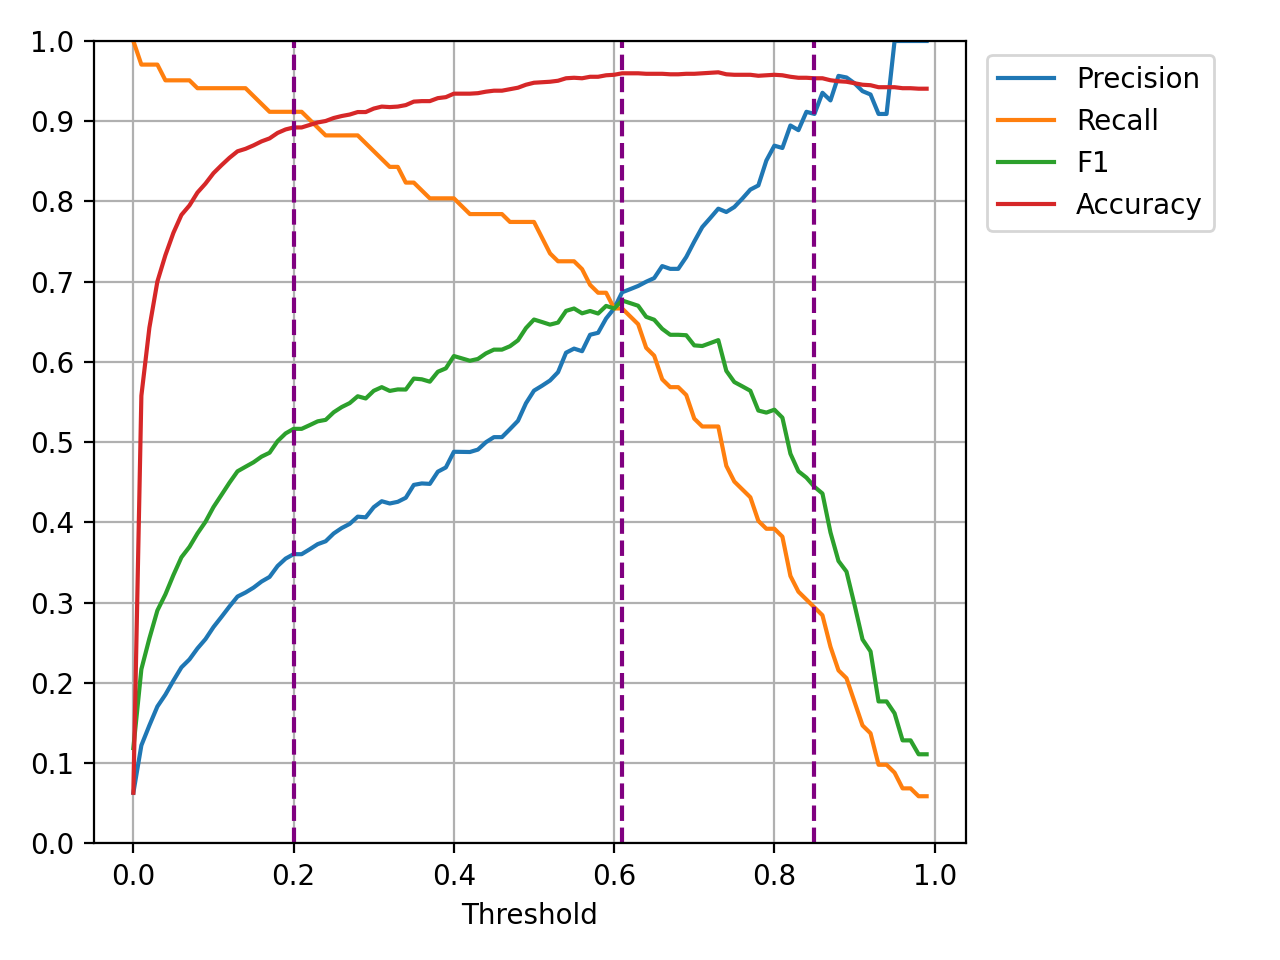
\includegraphics[width=.6\textwidth]{threshold_perf}
      \end{center}
    \end{frame}
    
    \begin{frame}
      \frametitle{Activity: computing performance metrics}

      Given the confusion matrix, find $\mc{P}$, $\mc{R}$ and $F_{1}$:

      \pause
      \begin{center} 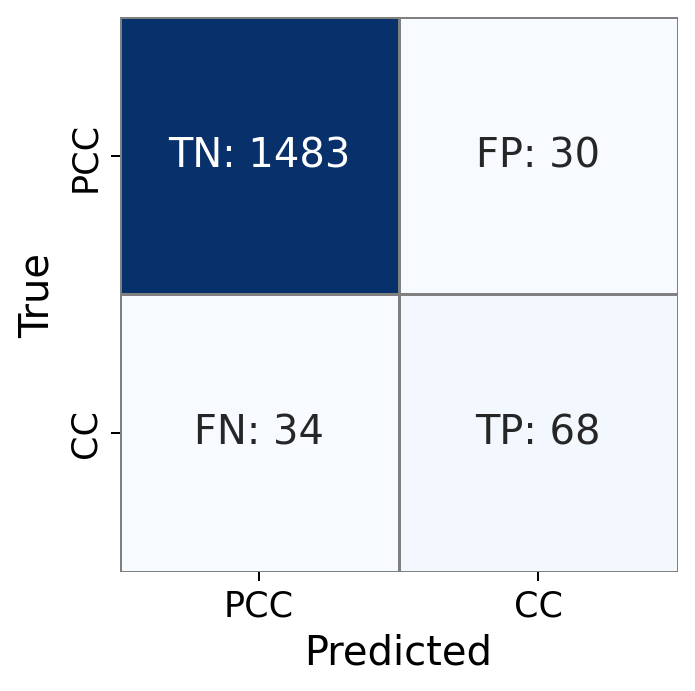
\includegraphics[width=.5\textwidth]{confusion_matrix_etc_th_0.61.png}
      \end{center}
      
    \end{frame}
    
\begin{frame}
  \frametitle{Performance curves}
  \pause
  \begin{itemize}
  \item ROC curves: TPR versus FPR for various $\tau$

    \pause

  \item Precision-recall curves: $\mc{P}$ versus $\mc{R}$ for various $\tau$

    \pause
   
  \item ROC and PRC of 3 candidate models:
  \end{itemize}

  \pause

  \begin{center}
    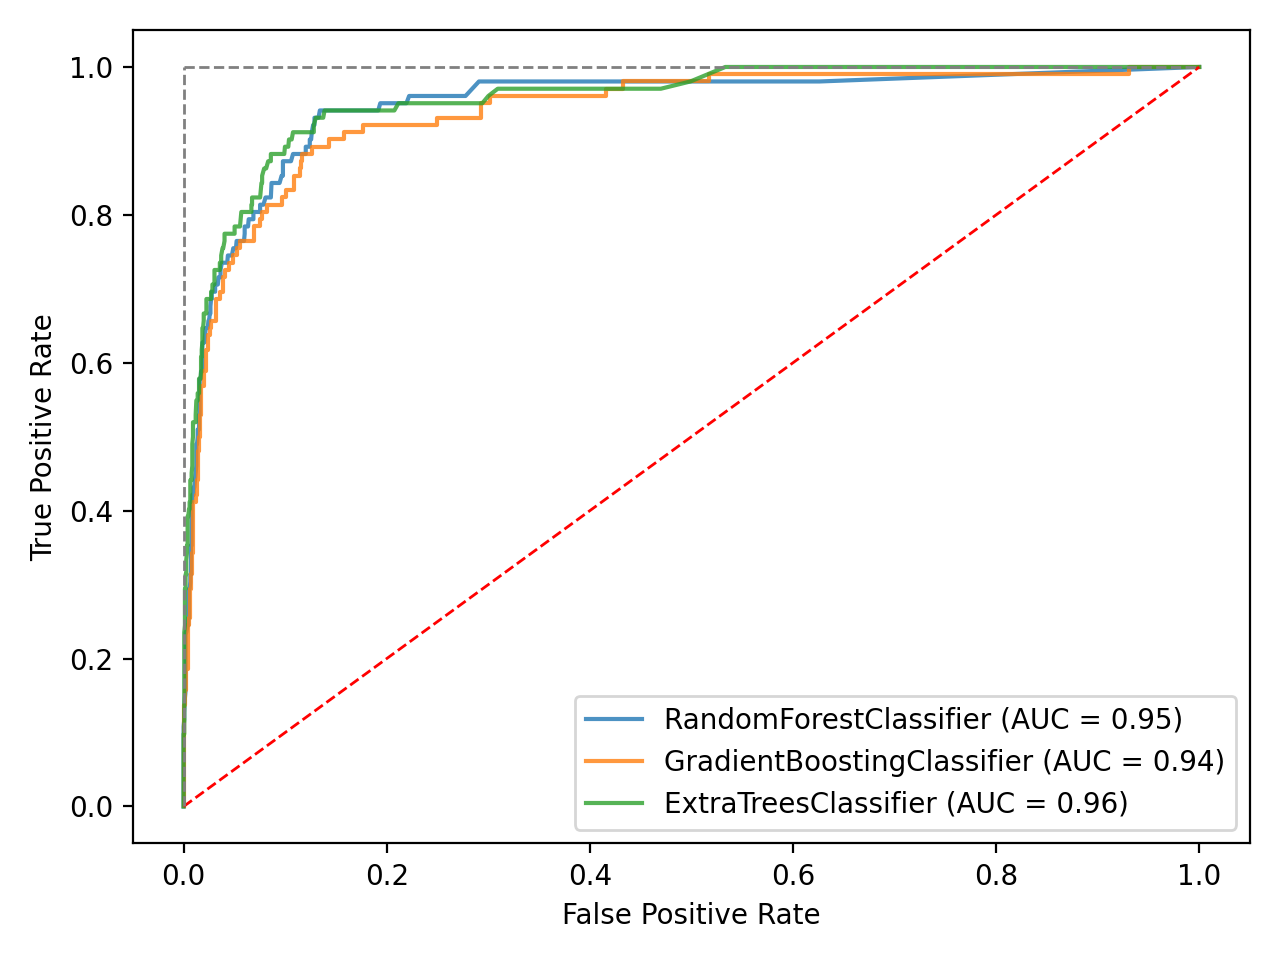
\includegraphics[width=.4\textwidth]{roc-all-models}
    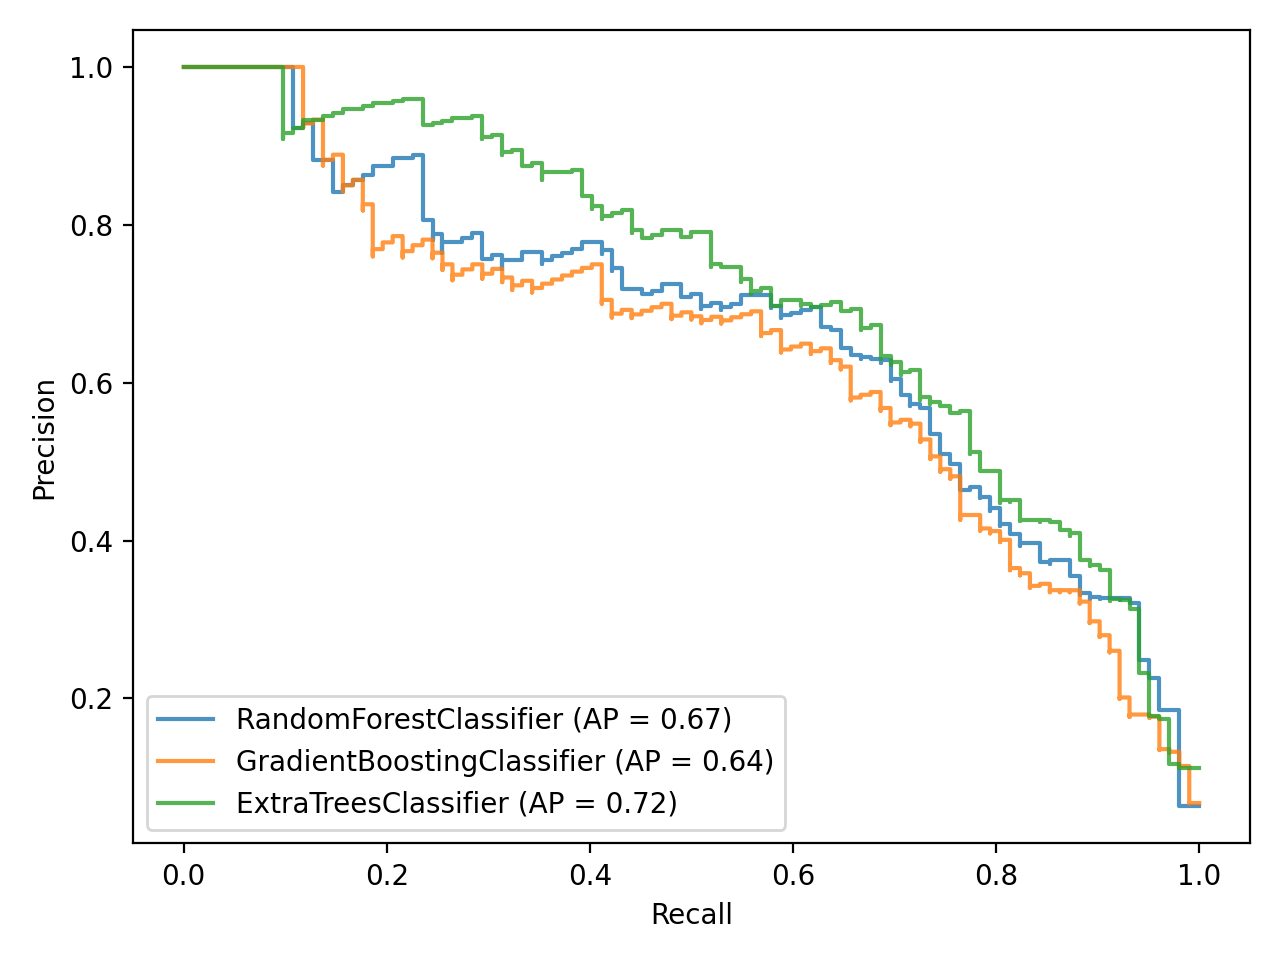
\includegraphics[width=.4\textwidth]{prc-all-models}
  \end{center}
\end{frame}


\begin{frame}
  \frametitle{Regression problems}
  \pause
  We find optimal parameters by minimizing loss functions such as:\pause
  \begin{itemize}
  \item L2 loss: squared error: $\ell_{2}(h,a) = (h-a)^{2}$\pause
  \item L1 loss: absolute value: $\ell_{2}(h,a) = |h-a|$\pause (robust to outliers)\pause
  \item Huber loss:
    \begin{equation}
      \ell_{\delta}(h,a) =
      \begin{cases}
        \fr{(h-a)^{2}}{2},          & |h-a|\le \delta \\
        \delta|h-a| - \delta^{2}/2, & |h-a| > \delta 
      \end{cases}
    \end{equation}
  \end{itemize}
  \pause

  \begin{center}
    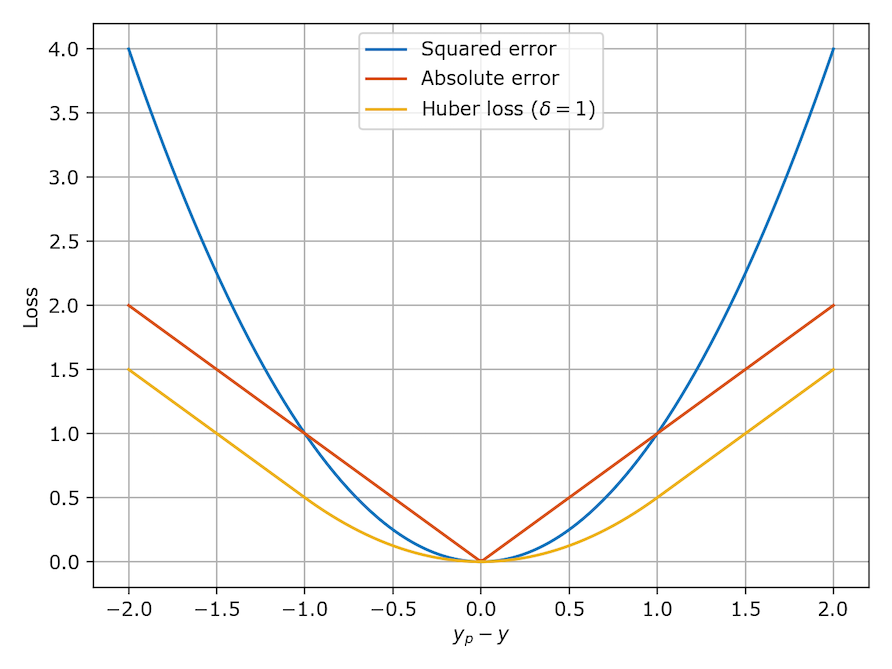
\includegraphics[width=.5\textwidth]{loss-functions.png}

    {\scriptsize Source: \url{https://www.evergreeninnovations.co/blog-machine-learning-loss-functions/}}
  \end{center}
  
\end{frame}


\section{Information theory}

\begin{frame}
  \frametitle{Entropy}
  \pause Entropy $\mathbb{H}$ is a measure of the lack of predictability (uncertainty) of a random variable $X$ with
  distribution $p$ over $K$ states: \pause

  \begin{equation}
    \mathbb{H}(X) \pause := -\sum_{k=1}^{K}p(X=k)\log_{2}p(X=k) \pause = -\expe_{X}[\log p(X)]
  \end{equation}

  \pause

  \begin{alertblock}{Notes}
    \begin{itemize}
    \item Entropy is measured in bits
      \pause
    \item For a $K$-ary r.v., entropy is maximized when $p(X=k) = \fr1K$
    \end{itemize}
    
  \end{alertblock}
\end{frame}

\begin{frame}
  \frametitle{Binary entropy function}
  \pause

  Binary r.v. $X\in \{0,1\}$; \pause $p(X=1) = \theta$; \pause $p(X=0) = 1 - \theta$. \pause

  \bigskip

  The binary entropy is given by:
  \pause
  \begin{align}
    \mb{H}(X) &=  -\sum_{k=1}^{K}p(X=k)\log_{2}p(X=k) \\
              &= -[p(X=1)\log_{2} p(X=1) + p(X=0)\log_{2}p(X=0)] \\
              &= -[\theta \log_{2}\theta + (1 - \theta)\log_{2}(1-\theta)]
  \end{align}
\end{frame}

\begin{frame}
  \frametitle{Multivariate entropy functions}
  \pause
  \begin{itemize}
  \item Cross entropy between distribution $p$ and $q$: \pause
    \begin{equation}
      \mb{H}(p,q) \pause := -\sum_{k=1}^{K} p_{k}\log q_{k}
    \end{equation}
    \pause

  \item Joint entropy of two r.v.'s $X$ and $Y$: \pause
    \begin{equation}
      \mb{H}(X,Y) \pause := -\sum_{x,y}p(x,y) \log_{2}p(x,y)
    \end{equation}

  \item Conditional entropy: \pause
    \begin{equation}
      \mb{H}(Y|X) \pause := \mb{H}(X, Y) - \mb{H}(X)
    \end{equation}

    \pause

  \item Chain rule for entropy: \pause
    \begin{equation}
      \mb{H}(X_{1}, X_{2}, \ldots, X_{n}) = \sum_{i=1}^{n}\mb{H}(X_{i}|X_{1}, \ldots, X_{i-1})
    \end{equation}
  \end{itemize}
\end{frame}

\begin{frame}
  \frametitle{Relative entropy}
  \pause

  Also known as the \textbf{Kullback-Leibler (KL) divergence} or \textbf{information gain}.\pause

  \bigskip

  It measures the dissimilarity (distance) between two distributions $p$ and $q$: \pause

  \begin{align}
    \mb{KL}(p||q)  & := \sum_{k=1}^{K} p_{k}\log\fr{p_{k}}{q_{k}} \quad \text{(Discrete)} \\\pause
    \mb{KL}(p||q)  & := \int p_{k}\log\fr{p_{k}}{q_{k}} dx \quad \text{(Continuous)} 
  \end{align}

  \pause

  In discrete case, we can show that: \pause
  \begin{equation}
     \mb{KL}(p||q) = \mb{H}(p,q) - \mb{H}(p)
  \end{equation}
  \pause
  i.e. cross entropy (between $p$ and $q$ minus entropy of $p$).
    
\end{frame}

\begin{frame}
  \frametitle{Entropy Venn diagrams}
  \pause

  \begin{center}
    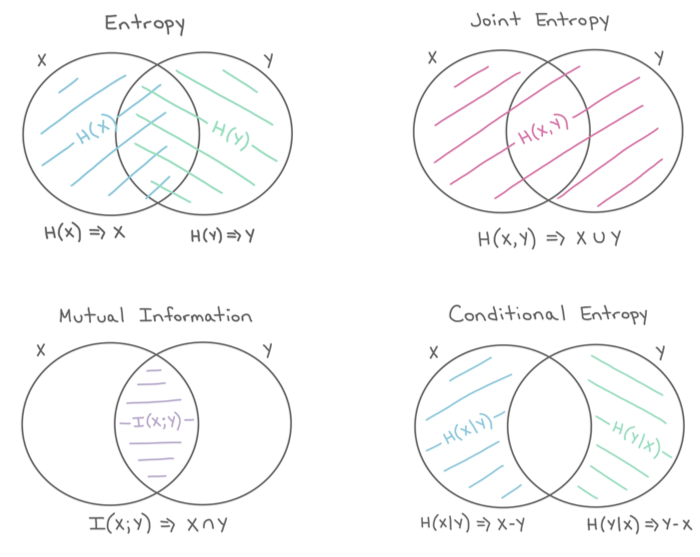
\includegraphics[width=.6\textwidth]{entropy-venn}

    {\scriptsize Source: PMLI Figure 6.4, page 211}
  \end{center}
\end{frame}

\begin{frame}
  \frametitle{Mutual information (MI)} 
  \pause
  This measures the dependency between two r.v.'s (more robust than correlation): \pause

  \begin{equation}
    \mb{I}(X;Y) := \mb{KL}(p(x,y)||p(x)p(y)) \pause = \sum_{y\in Y}\sum_{x\in X}p(x,y)\log\fr{p(x,y)}{p(x) p(y)}
  \end{equation}

  \pause

  \begin{alertblock}{}
    \begin{itemize}
    \item Can also be written as:
      \pause
      \begin{equation}
        \mb{I}(X;Y) = \mb{H}(X) - \mb{H}(X|Y) = \mb{H}(Y) - \mb{H}(Y|X)
      \end{equation}
      \pause

    \item MI is always $\ge 0$.
      \pause
    \item A normalized estimate of MI is the ``maximal information coefficient'' (MIC):\pause
      \begin{equation}
        MIC(X,Y) = \max_{G}\fr{\mb{I}((X,Y)|_{G})}{\log||G||}
      \end{equation}
      where $G$ is the set of 2d grids
    \end{itemize}
  \end{alertblock}
\end{frame}

\section{Outlook}

\begin{frame}
  \frametitle{Reading assignments}

  \begin{itemize}
  \item \textbf{PMLI} 5.1--5.4; 6.1--6.3
  \item \textbf{ESL} 7.1--7.7, 7.10--12

  \end{itemize}
\end{frame}

 
\appendix\addtocounter{part}{-1}

 
\section{Appendix}
 

\end{document}

%%% Local Variables:
%%% mode: latex
%%% TeX-master: t
%%% End:
